%
% $Id: $
%
%
% Compilar a .pdf con LaTeX (pdflatex)
% Es necesario instalar Beamer (paquete latex-beamer en Debian)
%

%
% Gráficos:
% Los gráficos pueden suministrarse en PNG, JPG, TIF, PDF, MPS
% Los EPS deben convertirse a PDF (usar epstopdf)
%

\documentclass{beamer}
\usetheme{GSyC}
%\usepackage[spanish]{babel}
\usepackage[latin1]{inputenc}
\usepackage{graphics}
\usepackage{amssymb} % Simbolos matematicos

%\definecolor{libresoftgreen}{RGB}{162,190,43}
%\definecolor{libresoftblue}{RGB}{0,98,143}

%\setbeamercolor{titlelike}{bg=libresoftgreen}

%% Metadatos del PDF.
\hypersetup{
  pdftitle={Teoría Tema 3 - Session Initiation Protocol},
  pdfauthor={Gregorio Robles},
  pdfcreator={GSyC, Universidad Rey Juan Carlos},
  pdfproducer=PDFLaTeX,
  pdfsubject={Teoría Tema 3 - Session Initiation Protocol},
}
%%

\begin{document}

\title{Teoría Tema 3 - Session Initiation Protocol}
\subtitle{Protocolos para la Transmisión de Audio y Vídeo en Internet}
\institute{grex@gsyc.urjc.es \\
GSyC, Universidad Rey Juan Carlos}
\author{Gregorio Robles}
\date[Oct 2014]{8 de octubre de 2014}

\frame{
\maketitle
}


% Si el titulo o el autor se quieren acortar para los pies de página
% se pueden redefinir aquí:
%\title{Titulo corto}
%\author{Autores abreviado}


%% LICENCIA DE REDISTRIBUCION DE LAS TRANSPAS
\frame{
~
\vspace{4cm}

\begin{flushright}
{\tiny
(cc) 2008-14 Jesús M. González Barahona, Gregorio Robles \\
  Some rights reserved. This work licensed under Creative Commons \\
  Attribution-ShareAlike License. To view a copy of full license, see \\
\ \\
  http://creativecommons.org/licenses/by-sa/3.0/ or write to \\
  Creative Commons, 559 Nathan Abbott Way, Stanford, \\
  California 94305, USA. \\

}
\end{flushright}
}
%%

\section{SIP: Session Initiation Protocol}

\begin{frame}
\frametitle{Introducción}

\begin{itemize}
\item Session Initiation Protocol: iniciación de sesiones sobre IP
\item RFC 2543 (SIP 2.0), RFC 3261 (clarified SIP 2.0)
\item Protocolo de señalización: prepara el establecimiento de
  sesiones multimedia
\item Concepto amplio de sesión: una llamada entre dos, una
  videoconferencia, un juego interactivo entre varios, etc.
\item Protocolo en evolución (mediante adiciones)
\item Usado en Internet, 3GPP
\item En VoIP compite con H.323 (IETF frente a ITU, en cierta medida)
\end{itemize}

\end{frame}

%%%%%%%%%%%%%%%%%%%%%%%%%%%%%%%%%%%%%%%%%%%%%%%%%%%%%%%%%%%%%%%%%%%%%%%

\begin{frame}
\frametitle{Principales características}

\begin{itemize}
\item Ligero (sólo seis métodos)
\item Basado en texto (similar a HTTP)
\item Independiente del nivel de transporte (TCP, UDP, ATM, etc.)
\item Se encarga del establecimiento y la terminación de la
  comunicación
\item Fundamentalmente es un protocolo peer-to-peer, aunque tiene servidores
\item Protocolo sin estado
\item Puerto habitual: 5060
\end{itemize}

\end{frame}

%%%%%%%%%%%%%%%%%%%%%%%%%%%%%%%%%%%%%%%%%%%%%%%%%%%%%%%%%%%%%%%%%%%%%%%

\begin{frame}
\frametitle{Relación con otros protocolos}

\begin{itemize}
\item Protocolo portador para descripciones SDP
\item Protocolo señalizador para RTP
\item Funcionalidad parcialmente similar a H.323
\item Hasta cierto punto equivalente a SS7, pero para VoIP
\end{itemize}

\end{frame}

%%%%%%%%%%%%%%%%%%%%%%%%%%%%%%%%%%%%%%%%%%%%%%%%%%%%%%%%%%%%%%%%%%%%%%%

\begin{frame}
\frametitle{Elementos de red}

\begin{itemize}
\item Terminales o \emph{user agents} (usualmente, los que establecerán la
  comunicación): Pueden comunicarse directamente, sin más elementos
\item Proxy: intermediarios que autentican, encaminan peticiones de
  llamada, etc
\item Registrar: permite informar de la localización actual
\item Redirect: genera redirecciones a peticiones, de manera que dirige las peticiones al siguiente servidor.
\end{itemize}

\end{frame}

%%%%%%%%%%%%%%%%%%%%%%%%%%%%%%%%%%%%%%%%%%%%%%%%%%%%%%%%%%%%%%%%%%%%%%%

\begin{frame}
\frametitle{Peticiones}

\begin{itemize}
\item INVITE: invitación a sesión
\item ACK: confirmación de respuesta a INVITE
\item BYE: terminación de sesión
\item CANCEL: cancela peticiones, pero no termina la sesión
\item OPTIONS: pregunta las capacidades de los servidores
\item REGISTER: registra la dirección con un registrar
\end{itemize}

\end{frame}

%%%%%%%%%%%%%%%%%%%%%%%%%%%%%%%%%%%%%%%%%%%%%%%%%%%%%%%%%%%%%%%%%%%%%%%

\begin{frame}
\frametitle{Cabeceras}

\begin{itemize}
\item {\bf Via}: muestra el protocolo de transporte y la ruta de la petición. Cada proxy añade una línea a este campo
\item {\bf From}: muestra la dirección del que llama.
\item {\bf To}: muestra la dirección del llamado.
\item {\bf Call-Id}: Identificador único para cada llamada; contiene la dirección del host. Será la misma para todos los mensajes en una misma sesión.
\item {\bf Cseq}: empieza con un número aleatorio y define de manera secuencial cada mensaje.
\item {\bf Contact}: Muestra una o más direcciones que pueden ser utilizadas para contactar al usuario
\item {\bf User Agent}: nombre de la aplicación cliente
\end{itemize}

\end{frame}


%%%%%%%%%%%%%%%%%%%%%%%%%%%%%%%%%%%%%%%%%%%%%%%%%%%%%%%%%%%%%%%%%%%%%%%

\begin{frame}[fragile]
\frametitle{Peticiones}

\begin{footnotesize}
\begin{verbatim}
Via: SIP/2.0/UDP 192.168.0.100:5060;rport;
     branch=z9hG4bK646464100000000b43c52d6c00000d1200000f03
Content-Length: 0
Contact: <sip:20000@192.168.0.100:5060>
Call-ID: ED9A8038-A29D-40AB-95B1-0F5F5E905574@192.168.0.100
CSeq: 36 REGISTER
From: <sip:20000@192.168.0.101>;tag=910033437093
Max-Forwards: 70
To: <sip:20000@192.168.0.101>
User-Agent: SJphone/1.60.289a (SJ Labs)
Authorization: Digest username="20000",realm="192.168.0.101",
               nonce="43c52e9d29317c0bf1f885b9aaff1522d93c7692",
               uri="192.168.0.101",
               response="f69463b8d3efdb87c388efa9be1a1e63"
\end{verbatim}
\end{footnotesize}

\end{frame}


%%%%%%%%%%%%%%%%%%%%%%%%%%%%%%%%%%%%%%%%%%%%%%%%%%%%%%%%%%%%%%%%%%%%%%%

\begin{frame}
\frametitle{Respuestas (ejemplos)}

\begin{itemize}
\item 1xx: información (180: llamando)
\item 2xx: éxito (200: OK)
\item 3xx: redirección (302: movimiento temporal)
\item 4xx: fallo (404: usuario no encontrado)
\item 5xx: fallo del servidor (500: error interno del servidor)
\item 6xx: fallo global
\end{itemize}

\end{frame}


%%%%%%%%%%%%%%%%%%%%%%%%%%%%%%%%%%%%%%%%%%%%%%%%%%%%%%%%%%%%%%%%%%%%%%%

\begin{frame}[fragile]
\frametitle{Respuesta (ejemplo)}

\begin{footnotesize}
\begin{verbatim}
Internet Protocol, Src Addr: 192.168.0.101 (192.168.0.101), Dst Addr:
192.168.0.100 (192.168.0.100)
User Datagram Protocol, Src Port: 5060 (5060), Dst Port: 5060 (5060)
Session Initiation Protocol
Status-Line: SIP/2.0 200 OK
Status-Code: 200
Resent Packet: False
Via: SIP/2.0/UDP 192.168.0.100:5060;rport;
     branch=z9hG4bK646464100000000b43c52d6c00000d1200000f03
Content-Length: 0
Contact: <sip:20100@192.168.0.100:5060>
Call-ID: ED9A8038-A29D-40AB-95B1-0F5F5E905574@100.100.100.16
CSeq: 36 REGISTER
From: <sip:20000@192.168.0.101>;tag=910033437093
Max-Forwards: 70
To: <sip:20000@192.168.0.101:5060>
Authorization: Digest username="20100",realm="192.168.0.101",
               nonce="43c52e9d29317c0bf1f885b9aaff1522d93c7692",
               uri="sip:192.168.0.101",
               response="f69463b8d3efdb87c388efa9be1a1e63"

\end{verbatim}
\end{footnotesize}

\end{frame}


%%%%%%%%%%%%%%%%%%%%%%%%%%%%%%%%%%%%%%%%%%%%%%%%%%%%%%%%%%%%%%%%%%%%%%%

\begin{frame}
\frametitle{Problemas con los NATs y firewalls}

\begin{itemize}
\item Los firewalls tienen que, al menos, tener el puerto 5060 abierto (y no filtrar paquetes UDP).
\item Tipos de NATs:
\begin{itemize}
  \item Full cone NATs: cualquiera puede enviar paquetes a nuestra máquina.
  \item Address-Restricted cone NAT: sólo pueden enviar paquetes a nuestra máquina aquéllos a los que les hemos enviado paquetes con anterioridad (misma IP)
  \item Port-Restricted cone NAT: sólo pueden enviar paquetes a nuestra máquina aquéllos a los que les hemos enviado paquetes con anterioridad (misma IP y mismo puerto)
  \item Symmetric NAT: Si se manda un paquete con la misma dirección interna y puerto a un destino diferente se usará un mapeo diferente. Sólo el host externo que recibe un paquete puede mandar un paquete UDP de vuelta al host interno.
\end{itemize}
\end{itemize}

\end{frame}



%%%%%%%%%%%%%%%%%%%%%%%%%%%%%%%%%%%%%%%%%%%%%%%%%%%%%%%%%%%%%%%%%%%%%%%

\begin{frame}
\frametitle{Ejemplo de una sesión}

\begin{center}
  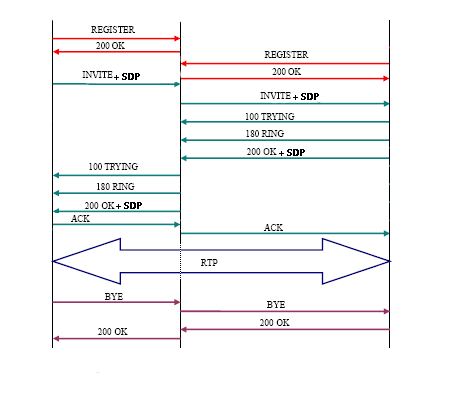
\includegraphics[width=6.6cm]{figs/complete-sip-session.png}
\end{center}

En los puntos finales, hay un \emph{user agent}. Entre medias, tenemos un servidor que actúa de \emph{Registrar} y \emph{Proxy}.

\end{frame}



%%%%%%%%%%%%%%%%%%%%%%%%%%%%%%%%%%%%%%%%%%%%%%%%%%%%%%%%%%%%%%%%%%%%%%%

\begin{frame}
\frametitle{Ejemplos de aplicaciones que usan SIP}

Terminales:
\begin{itemize}
\item Ekiga, WengoPhone
\item MS Windows Messenger
\item Apple iChat AV
\end{itemize}

Servidores (proxys, registrars):
\begin{itemize}
\item Asterisk
\end{itemize}

\end{frame}


%%%%%%%%%%%%%%%%%%%%%%%%%%%%%%%%%%%%%%%%%%%%%%%%%%%%%%%%%%%%%%%%%%%%%%%

\begin{frame}
\frametitle{Referencias}

\begin{itemize}
\item RFC 3261 \\
  \url{http://tools.ietf.org/html/rfc3261}
\item ``Session Initiation Protocolo'' (Wikipedia) \\
  \url{http://en.wikipedia.org/wiki/Session_Initiation_Protocol}
\item ``What is SIP'' \\
  \url{http://www.sipcenter.com/sip.nsf/html/What+Is+SIP+Introduction}
\item ``SIP Architecture'' \\
  \url{http://www.en.voipforo.com/SIP/SIP_architecture.php}
\end{itemize}

\end{frame}




\frame{
\maketitle
}

\end{document}
